\subsection{Energispektrum}
\label{sec:energispektrum}


\begin{figure}[h!]
  \centering
  \subbottom[Dobbelkoincidenser]{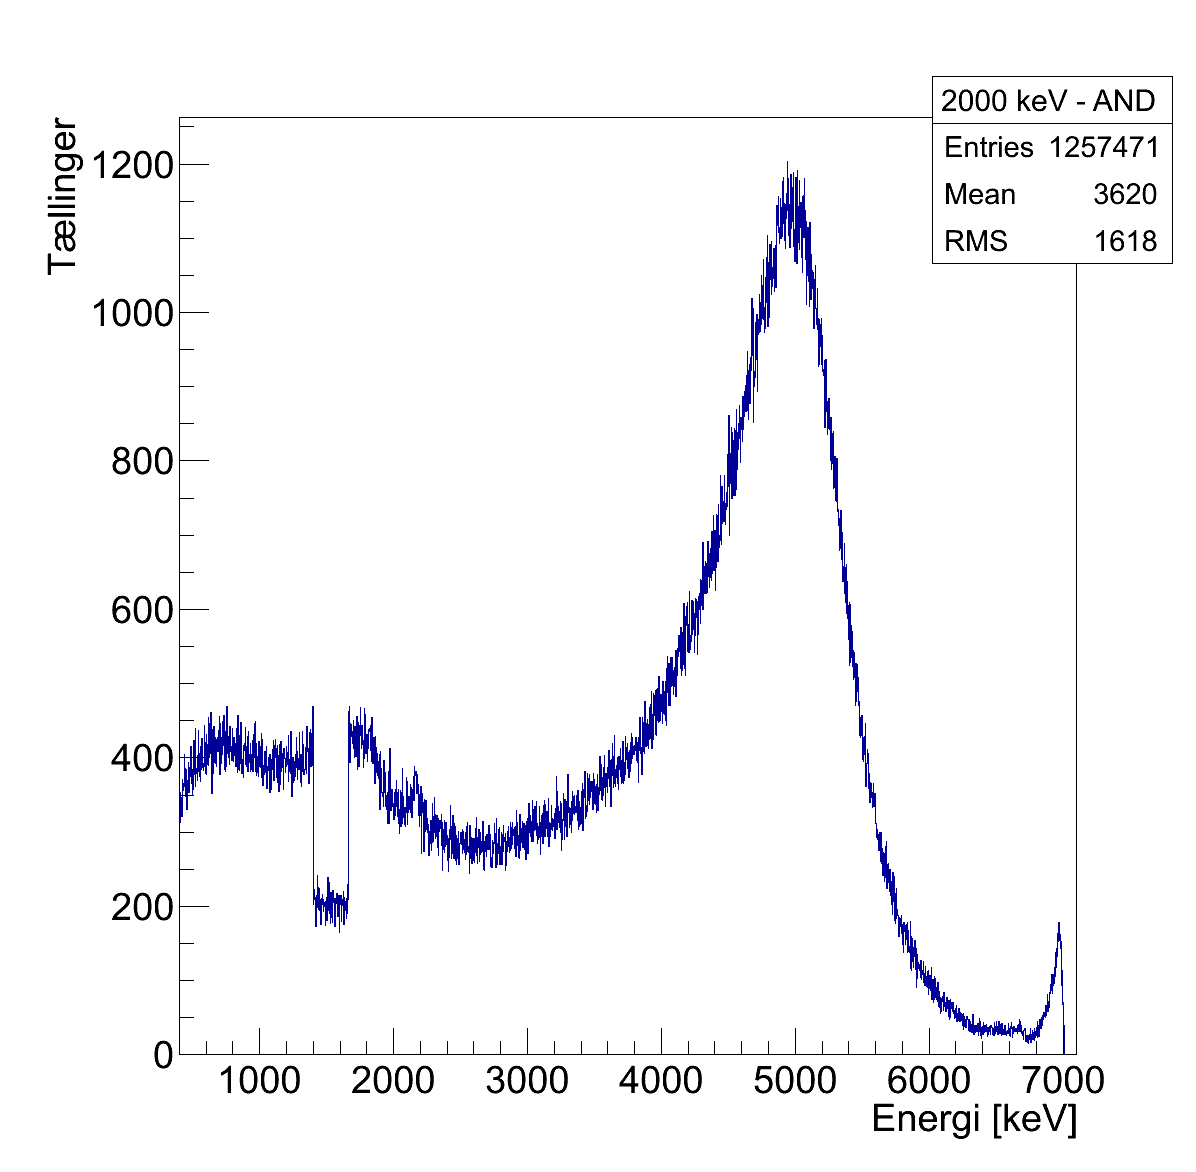
\includegraphics[width=0.46\columnwidth]{1077-spec-D}}%
  \hfill
  \subbottom[Trippelkoincidenser]{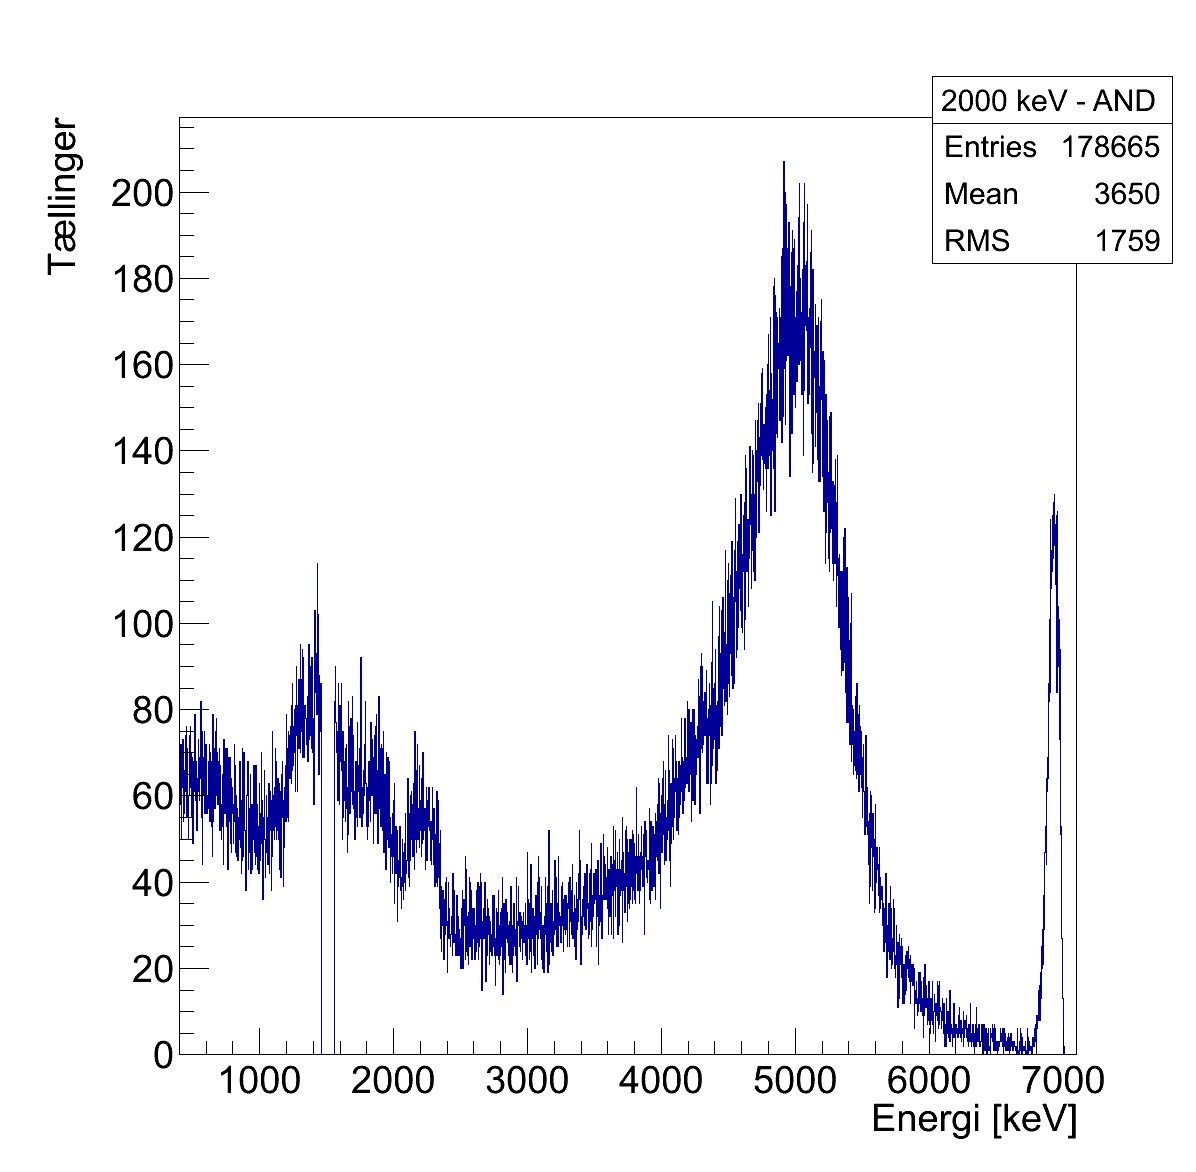
\includegraphics[width=0.46\columnwidth]{1077-spec-T}}%
  \caption{Antal tællinger som funktion af energien for henfald fra \SI{17.8}{\MeV}. Den smalle
    $\alpha_{0}$ og den brede $\alpha_{1}$ top ses tydeligt. Energierne ml. 1400 og 1660\keV er ikke medtaget
    i dobbelkoincidenser. Tilsvarende er 1460 og 1560\keV udeladt for trippelkoincidenserne.}
  \label{fig:alphaSpectrum}
\end{figure}

På \cref{fig:alphaSpectrum} ses alphaspektret i CM for hhv. dobbelt- og trippelkoincidenser, hvor
der er benyttet 2\MeV protoner. Dette populerer en $0^{+}$ tilstand i \Carb med excitations
energi  \SI{17.8}{\MeV}. Idet $\alpha$-henfald bevarer både impulsmoment og paritet, kan henfaldet
foregå både til grundtilstanden og den exciterede tilstand i beryllium. \fxfatal{Flyt til teori
  afsnit og uddyb. Se Hans' tegning. }
\fxfatal{Forklar sammenhæng ml. beamenergien og exitationsenergien af \Carb}

Først og fremmest skal det nævnes, at hvis energien af en af de detekterede $\alpha$-partikler lå mellem
1400 og 1660\keV, så er disse ikke medtaget i dobbelkoincidenserne, da dette gav anledning til
støj. Det samme gør sig gældende for trippelkoincidenserne mellem 1460 og 1560\keV.

I toppen af begge spektrer ses tydeligt en smal top omkring 7\MeV. Under denne ligger der en bred
Breit-Wigner lignende top centreret omkring 5\MeV. Disse toppe stemmer fint overens, både
mht. bredde og energi, med hvad det forventes for $\alpha_{0}$ og $\alpha_{1}$. $\alpha_{1}$-toppen er dog ikke
perfekt Breit-Wigner fordelt, hvilket bla. kan forklares ved, at der forekommer en bidrag fra de 
sekundære partikler.
\fxnote{Fordelingen afhænger også af energien af $\alpha$, som varierer henover toppen. }
Fordelingen af disse er det dog ikke muligt at sige noget videre meningsfuldt
om. Dette skyldes bidrag fra protonstrålen jvf. diskussion i \cref{cha:rutherford}.
\fxfatal{Sørg for at denne reference giver mening.}

De målte spektre er dermed i overenstemmelse med hypotesen om sekventielt henfald til tre
$\alpha$-partikler via \Be. Det essentiele spørgsmål er, om det er muligt at stole på de to
spektre.

Ud fra diskutionen i \cref{sec:sekv-kinematik} især med \cref{eq:Ealpha2} og \cref{eq:sekv-vinkel}
i mente, så ses at energien til rådighed for de sekundære $\alpha$-partikler i den transversale retning
afhænger af Q-værdien af det sekundære henfald.

Et henfald fra grundtilstanden af beryllium til tre $\alpha$-partikler frigører cirka 90\keV, hvorimod et
henfald fra den exciterede tilstand frigører omkring 3\MeV. Dette betyder, at den transversale
komposant af hastigheden af de sekundære $\alpha$-partikler kan være mange gange større, hvilket betyder
at vinklen mellem de to sekundære $\alpha$-partikler kan være tilsvarende større. Benytter man
\cref{eq:sekv-vinkel}, så er den maksimale vinkel hhv. \SI{19}{\degree} og \SI{86}{\degree} for
henfald til grundtilstanden og den exciterede tilstand.

\fxfatal{Dette skal gennemtænkes.}
Med det benyttede dektorsystem er der ikke fuld dækning i alle retninger, men fordi detektorerne er
placeret symmetrisk, så er detektorerne mere effektive til at detektere hændelser med lille vinkel
mellem de sekundære $\alpha$-partikler, da disse to ofte ville ramme samme detektor. Derimod er sandsynligheden
større for at kun to $\alpha$-partikler bliver detekteret, hvis vinklen er større, da der så er mulighed
for at en af partiklerne slet ikke detekteres.

Hvad betyder dette for koincidensspektrene? Effekten er tydeligst ved dobbeltkoincidenserne. Her
undertrykkes $\alpha_{0}$ kraftigst i forhold til $\alpha_{1}$. Dette skyldes, som beskrevet ovenfor, at der
vil være forholdvis flere hændelser, der skyldes henfald til den exciterede tilstand, hvor \emph{kun} to
partikler detekteres. Ved specifik at vælge disse hændelser undertrykkes $\alpha_{0}$-toppen.

Hvorfor er $\alpha_{1}$ så ikke undertrykt i trippelkoincidensspektret? Her er der to effekter, som
spiller ind. For det første er vinklen mellem detektorerne i størrelsesordnen 20\degree, hvilket
betyder, at der er en risiko for at begge sekundære partikler for $\alpha_{0}$ henfaldet rammer ved siden
af. Muligheden for større vinkel ved $\alpha_{1}$ henfald betyder også, at der er mulighed for, at
$\alpha$-partiklerne rammer hver sin detektor. Hvordan disse effekter har indflydelse på spektret er svær
at afgøre, men generelt er sandsynligheden for dektektere $\alpha_{1}$ tripler mindre end den for
$\alpha_{0}$. Forklaringen må af den grund være, at der simpelthen foregår flere
$\alpha_{1}$-henfald. Dette virker umiddelbart mærkeligt idet tunneleringssandsynligheden for
$\alpha$-henfald afhænger kraftigt af energien. Dette er nært relateret til levetiden og et udtrykt for
denne er udledt i \cite[s. 236]{Martin}
\begin{equation}
  \label{eq:SStunnel}
  \lambda \propto w(\alpha) e^{-G}, \qquad G \propto \frac{Z}{\sqrt{E_{\alpha}}}.
\end{equation}
Umiddelbart taler dette også for henfald med $\alpha_{0}$, men faktoren $w(\alpha)$ skal dog bemærkes. Dette
er en "fittefaktor" for at få teorien til at passe med de eksperimentelle data. Faktoren angiver
sandsynlighen for at finde $\alpha$-partiklen inden for kernen. Foltolkningen af
trippelkoincidensspektret er derfor, at det er mere sandsynligt, at $\Carb(\SI{17.8}{\MeV})$ består
beryllium i en $2^{+}$ tilstand sammen med en $L=2$ $\alpha$-partikel, end $0^{+}$ beryllium sammen med
en $L=0$ $\alpha$-partikel. Dette stemmer overens med de tabulerede værdier af tværsnittet i
\cite{States}, der angiver værdierne $\sigma(\alpha_{0}) = \SI{9}{\ub}$ og
$\sigma(\alpha_{1}) = \SI{25}{\ub}$. Værdien for tværsnittet af $\alpha_{1}$-processen er dog mere usikker.

% Dette skyldes at der er tale om
% en vinkeldistribution, som kan antage alle værdier mellem 0 og maksimalværdien. Dermed vil der
% forekomme sekundære partikler fra $\alpha_{1}$ henfald, hvor vinklen er lille. Desuden så er åbningerne
% imellem detektorerne i størrelsesorden 20\degree målt fra \target. Dermed er det muligt at begge
% sekundære partikler fra $\alpha_{0}$ ikke detekteres, hvorimod der er en sandsynlig for at de sekundære
% partikler rammer hver sin detektor, hvis der er tale om $\alpha_{1}$-henfald. Sidst men ikke mindt, skal
% det nævnes, at de sekundære $\alpha$-partikler bidrager til $\alpha_{1}$ toppen. 

Den præcise modulering af de to toppe er dermed meget afhængig hvilke koincidensbetingelser der
stilles, men afhænger også af den specifikke opstilling. For at opnå fuld forståelse af
fordelingen er det derfor nødvendigt at foretage en simulering. Dette ligger dog uden for tidsrammen
af dette projekt. Derfor vil dobbelt- og trippelkoincidenserne behandles separat i den videre
analyse. 